\section{Root-Zertifikate importieren}
Das Importieren der Zertifikate in Web-Browser und E-Mail-Client erspart l�stige Nachfragen, ob man einem mit diesem Root-Zertifikat signierten Zertifikat vertrauen m�chte.
\subsection{Webbrowser Firefox}
Nutzer des Browsers Firefox klicken auf auf das \textit{Root Certificate} und aktivieren in dem sich �ffnenden Dialog (Bild \ref{abb:firefox_ca_neu}) mindestens den ersten und zweiten Punkt.\\

\begin{figure}[htb]
 \begin{center}
  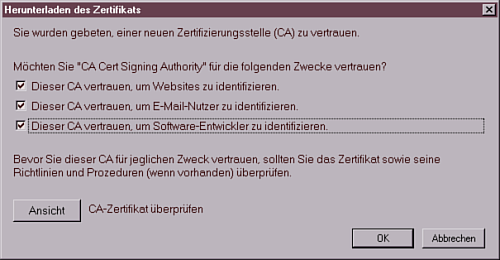
\includegraphics[scale=0.55]{../screenshots/cacert_certifikat.png}
  \caption{Herunterladen eines Zertifikates}
\label{abb:firefox_ca_neu}
 \end{center}
\end{figure}

\subsection{E-Mail-Client Thunderbird}
F�r den Import der Root-Zertifikate in den E-Mail-Client sind diese lokal zu speichern. In der Regel ben�tigt man neben dem \textit{Class 1 Root Certificate} auch das \textit{Class 3 Root Certificate}, da mit diesem Unterzertifikat die E-Mail-Zertifikate der Nutzer signiert werden. Nutzer des Browsers Firefox klicken mit der rechten Maustaste auf den Link und w�hlen aus dem Kontextmen� den Punkt \textit{Ziel speichern unter ...}\\

\begin{figure}[htb]
 \begin{center}
  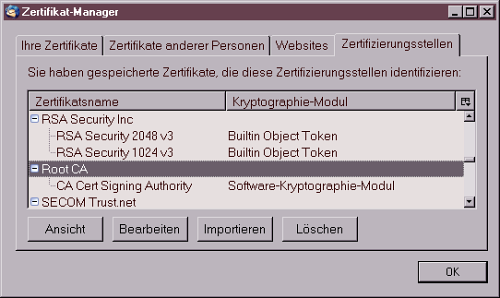
\includegraphics[scale=0.55]{../screenshots/thunderbird_zerti_manager.png}
  \caption{Zertifikats-Manager von Thunderbird}
\label{abb:thunder_ca_neu}
 \end{center}
\end{figure}

Anschlie�end ist Thunderbird zu starten und der Dialog \textit{Einstellungen} zu �ffnen. In der Sektion \textit{Datenschutz} / \textit{Sicherheit} ist der Button \textit{Zertifikate} zu w�hlen, um den in Bild \ref{abb:thunder_ca_neu} dargestellten Manager f�r Zertifikate zu �ffnen.\\

In diesem Dialog ist auf dem Reiter \textit{Zertifizierungsstellen} der Button \textit{Importieren} zu w�hlen und das zuvor gespeicherte Zertifikat zu importieren. Im Anschluss sind im folgenden Dialog mindestens die ersten beiden Optionen zu aktivieren (siehe Firefox).\\

\section{Eine eigene Certification Authority}
Wer eine eigene Certification Authority (CA) betreiben m�chte, ben�tigt etwas Erfahrung, einige kleine Tools und ein paar Byte Webspace, um das eigene Root-Zertifikate, die Revocation List und die Policy der CA dort zum Download bereitzustellen.\\

Die OpenSSL-Bibliothek enth�lt alle n�tigen Funktionen, um eine eigene CA zu verwalten. Die Hardcore Version auf der Kommandozeile hat M. Heimpold im Mini-Howto zur Zertifikatserstellung beschrieben.\\ \href{http://www.heimpold.de/mhei/mini-howto-zertifikaterstellung.htm}{http://www.heimpold.de/mhei/mini-howto-zertifikaterstellung.htm}.\\

Komfortabler geht es mit dem GUI TinyCA (\href{http://tinyca.sm-zone.net}{http://tinyca.sm-zone.net}). Die Website bietet eine Live-CD zum Download an, so dass ich mir weitere Ausf�hrungen zur Installation sparen kann. Unter Debian GNU/Linux kann man das Tool mit Apt installieren:

\begin{verbatim}
   # apt-get install tinyca
\end{verbatim}

Nach dem Start mit dem Kommando \textit{tinyca2} werden in zwei Dialogen die Angaben zum Root-Zertifikat der CA abgefragt. Da TinyCA mehrere CAs verwaltet, kann man erst einmal mit einem Test beginnen.\\

\begin{figure}[htb]
 \begin{center}
  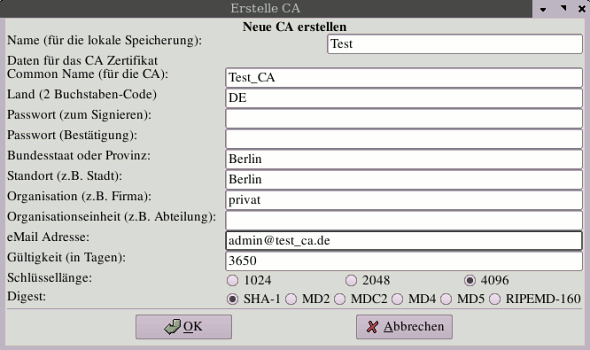
\includegraphics[scale=0.55]{../screenshots/tinyca1.png}
  \caption{Anlegen einer neuen CA}
\label{abb:tinyca1}
 \end{center}
\end{figure}

Der \textit{Common Name} der CA kann frei gew�hlt werden. Das Passwort sollte man sich gut �berlegen und keinesfalls vergessen. Mit einem Klick auf \textit{Ok} erscheint ein zweiter Dialog mit weiteren Angaben zur CA. Wichtig sind hier die URL der Revocation List f�r zur�ckgezogene Zertifikate und die URL der Policy der CA. Die Policy ist ein HTML-Dokument, welches beschreibt, wer ein Zertifikat von dieser CA erhalten kann, also z.B. etwas in der Art: \textit{Nur f�r pers�nlich Bekannte!}\\

Im Anschluss k�nnen die E-Mail Zertifikate der Nutzer erstellt werden. Die n�tigen Angaben sind selbsterkl�rend (Bild \ref{abb:tinyca3}. Mit einem Klick auf \textit{Ok} wird das S/MIME-Zertifikat erstellt und mit dem Root-Zertifikat der CA signiert. Dabei wird das Password f�r den geheimen Key der CA abgefragt.\\

\begin{figure}[htb]
 \begin{center}
  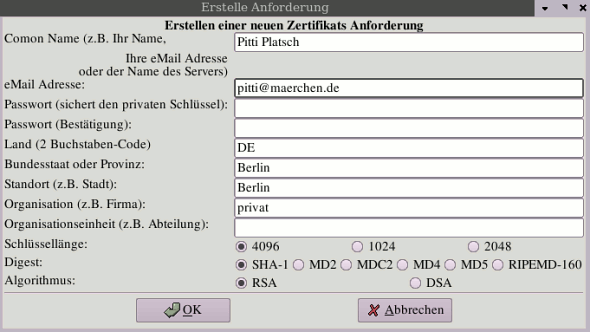
\includegraphics[scale=0.55]{../screenshots/tinyca3.png}
  \caption{Erstellen eines E-Mail Zertifikats}
\label{abb:tinyca3}
 \end{center}
\end{figure}

Um einem Nutzer sein Zertifikat zur Verf�gung zu stellen, ist es in eine Datei zu exportieren. Das PKCS\#12-Format (*.p12) enth�lt den geheimen und den �ffentlichen Schl�ssel, ist mit einem Passwort gesichert und kann von allen E-Mail Clients importiert werden.\\

\begin{figure}[htb]
 \begin{center}
  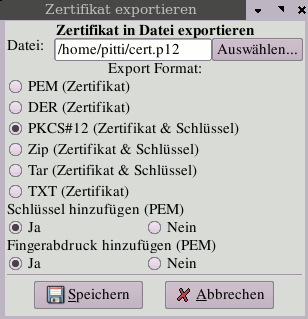
\includegraphics[scale=0.5]{../screenshots/tinyca5.png}
  \caption{Zertifikat exportieren}
\label{abb:tinyca5}
 \end{center}
\end{figure}

Das Root-Zertifikat der CA ist als DER- oder PEM-Format zu exportieren. Diese Datei enth�lt nur den �ffentlichen Schl�ssel des Zertifikates und kann zum Download bereitgestellt werden. Au�erdem ist regelm��ig eine Revocation List mit abgelaufenen oder zur�ckgezogenen Zertifikaten zu erstellen und ebenfalls zum Download unter der angegebenen URL bereitzustellen. Die Oberfl�che bietet f�r beide Aufgaben einen Button in der Toolbar.